\documentclass[aspectratio=169]{beamer}
\usetheme{metropolis} % Un tema moderno y limpio

\usepackage[utf8]{inputenc}
\usepackage[english]{babel}
\usepackage{booktabs}
\usepackage{graphicx}
\usepackage{tikz}
\usetikzlibrary{shapes.geometric, calc}
% Se añade 'positioning' a las librerías
\usetikzlibrary{shapes.geometric, calc, positioning, backgrounds}

\title{LLMs \& VLMs course}
\subtitle{Introduction to Large Language Models}
\author{Juan Irving Vasquez}
\date{\today}
\institute{Instituto Politécnico Nacional (IPN)}
\titlegraphic{
\includegraphics[height=1.2cm]{ipn-cidetec.png}\hspace{0.1cm}
\includegraphics[height=1.2cm]{escudoESCOM}}

\begin{document}

\maketitle

\frame{
	\frametitle{The A.I. revolution}
	\begin{columns}[c] % El parámetro [c] alinea el contenido verticalmente al centro
		
		% --- Columna Izquierda (Texto) ---
		\begin{column}{0.5\textwidth}
			\begin{itemize}
				\item ChatGPT became publicly available in November 30 2022\footnote{Gemini, Consulted May 26.}
				\item It reached 100 million users in just two months.
				\item 550 M in 2025.
			\end{itemize}
		\end{column}
		
		% --- Columna Derecha (Imagen) ---
		\begin{column}{0.5\textwidth}
			\begin{figure}
				\centering
				% Ajusté el ancho a \linewidth para que se adapte al tamaño de su columna
				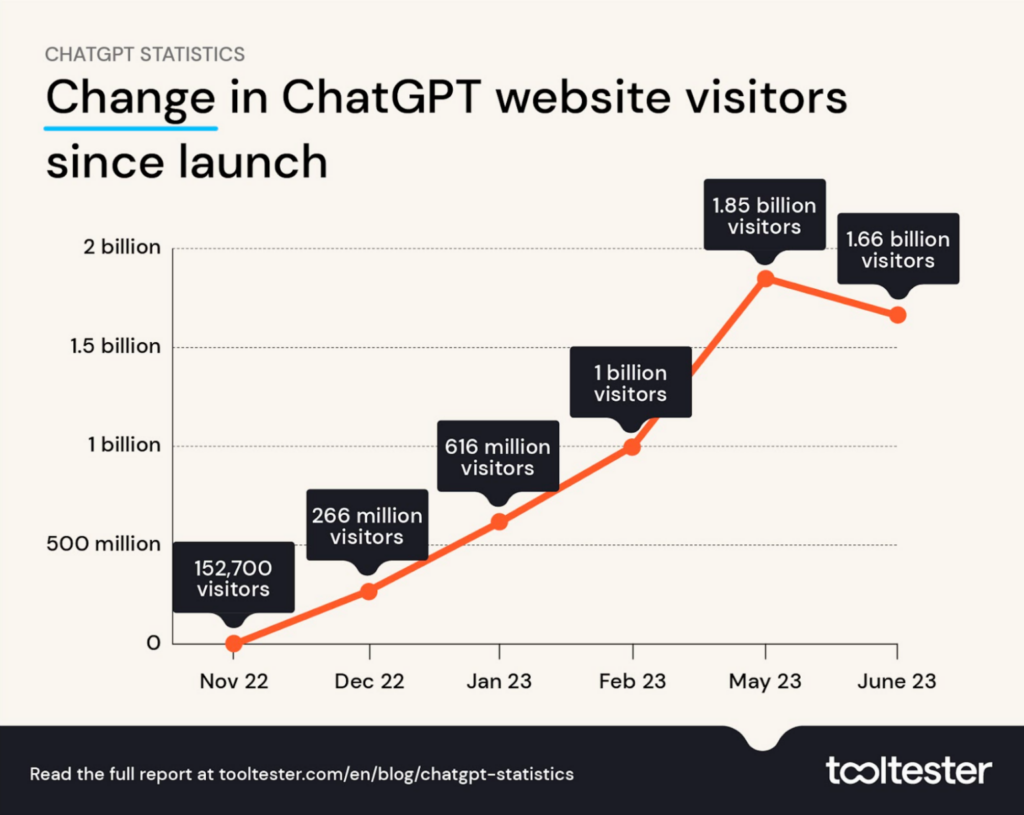
\includegraphics[width=\linewidth]{figures/chatgpt-user} 
				\caption{}
				\label{fig:chatgpt-user}
			\end{figure}
		\end{column}
	\end{columns}
}





% --- Hierarchical Context ---
\begin{frame}{AI Landscape}
	\begin{itemize}
		\item \textbf{Artificial Intelligence:} Systems capable of human-like intelligence tasks.
		\item \textbf{Machine Learning:} Algorithms that learn rules automatically from data (no explicit programming).
		\item \textbf{Deep Learning:} A subset of ML utilizing multi-layer neural networks.
		\item \textbf{Generative AI (GenAI):} Models designed to create new content (text, images, media).
		\item \textbf{LLMs:} Specific application of deep learning for parsing and generating human-like text.
	\end{itemize}
\end{frame}


% --- Slide 1: Introduction ---
\begin{frame}{The New Era of Natural Language Processing}
    \begin{itemize}
        \item \textbf{Traditional NLP:} Excelled at categorization (spam detection) and pattern recognition via handcrafted rules or shallow models.
        \item \textbf{The LLM Shift:} Modern models (e.g., ChatGPT) leverage deep neural networks to manage complex linguistic tasks.
        \item \textbf{Capabilities:} Understanding instructions, contextual analysis, and coherent text generation.
        \item \textbf{Key Insight:} "Understanding" in LLMs refers to statistical coherence and contextual relevance, not human-like consciousness.
    \end{itemize}
\end{frame}

% --- Slide 2: Defining LLMs ---
\begin{frame}{What is a Large Language Model (LLM)?}
    \begin{block}{Definition}
        An LLM is a deep neural network designed to "understand", generate, and respond to human-like text by being trained on massive datasets.
    \end{block}
    \begin{itemize}
        \item \textbf{"Large" dimensions:}
            \begin{itemize}
                \item \textbf{Parameter Size:} Often tens or hundreds of billions of weights optimized during training.
                \item \textbf{Dataset Scale:} Sometimes encompassing significant portions of the publicly available internet.
            \end{itemize}
        \item \textbf{Core Objective:} Next-word prediction (leveraging the sequential nature of language).
    \end{itemize}
\end{frame}




\begin{frame}[fragile]{Development}
	\begin{figure}
		\centering
		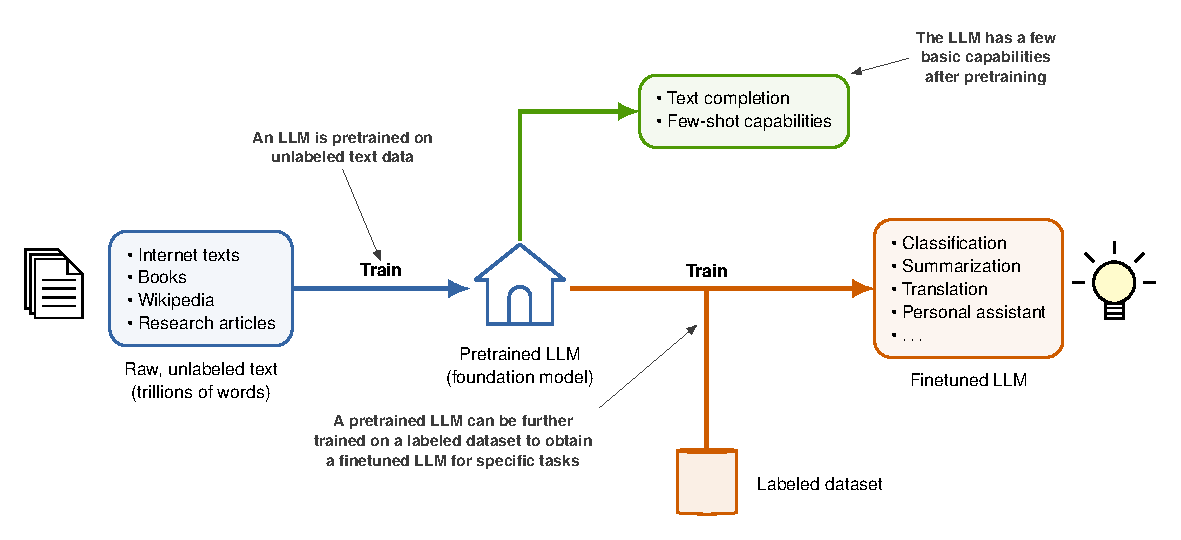
\includegraphics[width=0.93\linewidth]{./figures/llm_train}
		%\caption{}
		\label{fig:devel}
	\end{figure}
\end{frame}



% --- Slide 4: Pretraining vs. Finetuning ---
\begin{frame}{The Two-Stage Training Paradigm}
    LLM development typically follows a bifurcated process:
    \vspace{0.5cm}
    \begin{enumerate}
        \item \textbf{Pretraining (Self-Supervised):}
            \begin{itemize}
                \item Trained on large, unlabeled corpora (trillions of words).
                \item Result: \textbf{Foundation/Base Model} (e.g., GPT-3).
                \item Capability: Text completion and few-shot learning.
            \end{itemize}
        \vspace{0.3cm}
        \item \textbf{Finetuning (Supervised):}
            \begin{itemize}
                \item Narrow dataset specific to tasks or domains.
                \item \textbf{Instruction-finetuning:} Adapting for chat/assistants.
                \item \textbf{Classification-finetuning:} Specializing for sentiment or toxicity detection.
            \end{itemize}
    \end{enumerate}
\end{frame}


\begin{frame}
\frametitle{Transformer insight}
\begin{center}
	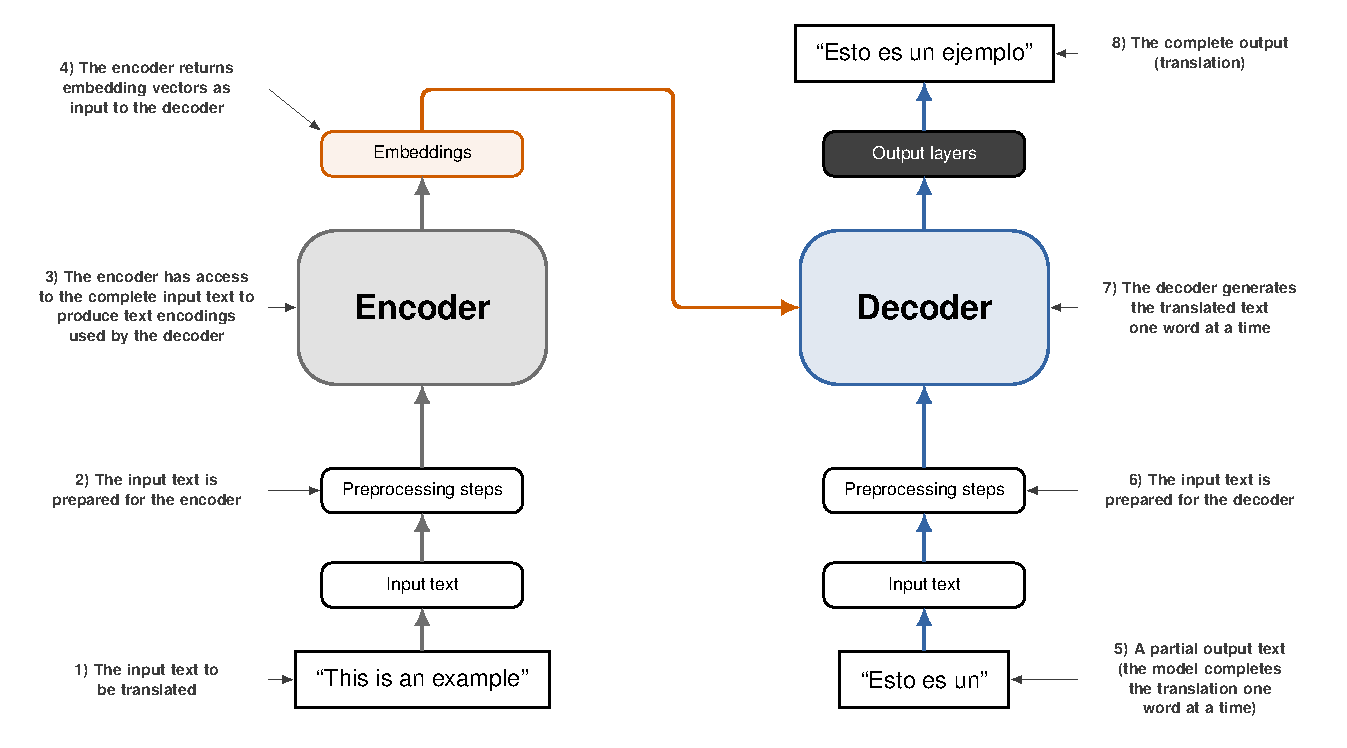
\includegraphics[width=0.9\linewidth]{figures/transformer_insight}
\end{center}
\end{frame}



% --- Slide 5: The Transformer Architecture ---
\begin{frame}{The Transformer Foundation}
    Most modern LLMs rely on the architecture introduced in \textit{"Attention Is All You Need"} (2017).
    \begin{itemize}
        \item \textbf{Encoder-Decoder:} Original design for machine translation (English $\rightarrow$ German).
        \item \textbf{Self-Attention Mechanism:} Allows the model to weigh the importance of different tokens in a sequence relative to each other, capturing long-range dependencies.
        \item \textbf{Architectural Variants:}
            \begin{itemize}
                \item \textbf{BERT:} Encoder-only; specialized in masked word prediction and classification.
                \item \textbf{GPT:} Decoder-only; specialized in generative tasks and autoregressive word prediction.
            \end{itemize}
    \end{itemize}
\end{frame}



% --- Slide 6: Utilizing Large Datasets ---
\begin{frame}{Scaling Laws: Data for LLMs}
    LLMs require diverse and comprehensive text corpora encompassing billions of words.
    \begin{table}[]
        \centering
        \caption{GPT-3 Pretraining Dataset (Sampled 300B Tokens)}
        \begin{tabular}{@{}lll@{}}
        \toprule
        \textbf{Dataset} & \textbf{Description} & \textbf{Proportion} \\ \midrule
        Common Crawl & Filtered web crawl (410B tokens) & 60\% \\
        WebText2 & Outbound Reddit links ($3+$ upvotes) & 22\% \\
        Books1/2 & Project Gutenberg / Libgen & 16\% \\
        Wikipedia & High-quality text (English) & 3\% \\ \bottomrule
        \end{tabular}
        \label{tab:gpt3_data}
    \end{table}
    \begin{itemize}
        \item \textbf{Cost:} GPT-3 pretraining estimated at \$4.6M in cloud credits.
    \end{itemize}
\end{frame}


% --- Slide 7: Emergent Behaviors ---
\begin{frame}{Emergent Behaviors and Multitasking}
    \begin{itemize}
        \item \textbf{Definition:} Capabilities not explicitly taught during training but arising as a natural consequence of large-scale data exposure.
        \item \textbf{Example:} GPT models can perform translation despite being trained primarily on next-word prediction.
        \item \textbf{Foundation Models:} Their versatile nature allows them to be used as general-purpose tools for tasks not seen in training data.
        \item \textbf{Advantage:} Custom-built LLMs (e.g., BloombergGPT) can outperform general LLMs in specific domains like finance.
    \end{itemize}
\end{frame}



% --- Slide 8: Implementation Plan ---
\begin{frame}{Building an LLM from Scratch}
    The roadmap for the implementation:
    \begin{itemize}
        \item \textbf{Stage 1: Data and Architecture:} Data preparation, tokenization (BPE), and coding the Attention mechanism.
        \item \textbf{Stage 2: Pretraining:} Implementing the training loop and evaluating performance (Educational scale).
        \item \textbf{Stage 3: Finetuning:} Taking a base model and adapting it for specific instruction-following or classification.
    \end{itemize}
\end{frame}


\begin{frame}{Bibliography}
	\begin{itemize}
		\item Raschka, Sebastian. Build a large language model (from scratch). Simon and Schuster, 2024.
		\item Goodfellow, Ian, et al. Deep learning. Vol. 1. No. 2. Cambridge: MIT press, 2016.
	\end{itemize}
\end{frame}

\begin{frame}[standout]
    Questions?
\end{frame}

\end{document}
